\documentclass[12pt,a4paper,bibliography=totocnumbered,listof=totocnumbered]{scrartcl}
\usepackage[ngerman]{babel}
\usepackage[utf8]{inputenc}
\usepackage{amsmath}
\usepackage{amsfonts}
\usepackage{amssymb}
\usepackage{graphicx}
\usepackage{fancyhdr}
\usepackage{tabularx}
\usepackage{geometry}
\usepackage{setspace}
\usepackage[right]{eurosym}
\usepackage[printonlyused]{acronym}
\usepackage{subfig}
\usepackage{floatflt}
\usepackage[usenames,dvipsnames]{color}
\usepackage{colortbl}
\usepackage{paralist}
\usepackage{array}
\usepackage{titlesec}
\usepackage{parskip}
\usepackage{acronym}
\usepackage[modulo]{lineno}
\pagewiselinenumbers
\usepackage{footmisc}
\usepackage[right]{eurosym}
\usepackage[subfigure,titles]{tocloft}
\usepackage[pdfpagelabels=true]{hyperref}

\usepackage{listings}
\lstset{basicstyle=\footnotesize, captionpos=b, breaklines=true, showstringspaces=false, tabsize=2, frame=lines, numbers=left, numberstyle=\tiny, xleftmargin=2em, framexleftmargin=2em}
\makeatletter
\def\l@lstlisting#1#2{\@dottedtocline{1}{0em}{1em}{\hspace{1,5em} Lst. #1}{#2}}
\makeatother

\geometry{a4paper, top=27mm, left=30mm, right=20mm, bottom=35mm, headsep=10mm, footskip=12mm}

\hypersetup{unicode=false, pdftoolbar=true, pdfmenubar=true, pdffitwindow=false, pdfstartview={FitH},
	pdftitle={Bachelorarbeit},
	pdfauthor={Fabian Wilms},
	pdfsubject={Bachelorarbeit},
	pdfcreator={\LaTeX\ with package \flqq hyperref\frqq},
	pdfproducer={pdfTeX \the\pdftexversion.\pdftexrevision},
	pdfkeywords={Bachelorarbeit},
	pdfnewwindow=true,
	colorlinks=true,linkcolor=black,citecolor=black,filecolor=magenta,urlcolor=black}
\pdfinfo{/CreationDate (D:20110620133321)}

\begin{document}

\titlespacing{\section}{0pt}{12pt plus 4pt minus 2pt}{-6pt plus 2pt minus 2pt}

% Kopf- und Fusszeile
\renewcommand{\sectionmark}[1]{\markright{#1}}
\renewcommand{\leftmark}{\rightmark}
\pagestyle{fancy}
\lhead{}
\chead{}
\rhead{\thesection\space\contentsname}
\lfoot{Generative Testerstellung für Microservice-Architekturen}
\cfoot{}
\rfoot{Seite \thepage}
\renewcommand{\headrulewidth}{0.4pt}
\renewcommand{\footrulewidth}{0.4pt}

% Vorspann
\renewcommand{\thesection}{\Roman{section}}
\renewcommand{\theHsection}{\Roman{section}}
\pagenumbering{Roman}

% ----------------------------------------------------------------------------------------------------------
% Titelseite
% ----------------------------------------------------------------------------------------------------------
\thispagestyle{empty}
\begin{center}
	\includegraphics[scale=0.25]{images/Hochschule_Muenchen_Logo.png}\\
	\vspace*{2cm}
	\Large
	\textbf{Fakultät für Informatik und Mathematik 07}\\
	\vspace*{2cm}
	\Huge
	\textbf{Bacheloararbeit}\\
	\vspace*{0.5cm}
	\large
	über das Thema\\
	\vspace*{1cm}
	\textbf{Generative Testerstellung für Microservice-Architekturenit}\\
	\vspace*{2cm}
	
	\vfill
	\normalsize
	\newcolumntype{x}[1]{>{\raggedleft\arraybackslash\hspace{0pt}}p{#1}}
	\begin{tabular}{x{6cm}p{7.5cm}}
		\rule{0mm}{5ex}\textbf{Autor:} & Fabian Wilms\newline holtkoet@hm.edu \\ 
		\rule{0mm}{5ex}\textbf{Prüfer:} & Prof. Dr. Ulrike Hammerschall \\ 
		\rule{0mm}{5ex}\textbf{Abgabedatum:} & xx.xx.2017 \\ 
	\end{tabular} 
\end{center}
\pagebreak

% ----------------------------------------------------------------------------------------------------------
% Abstract
% ----------------------------------------------------------------------------------------------------------
\setcounter{page}{1}
\onehalfspacing
\titlespacing{\section}{0pt}{12pt plus 4pt minus 2pt}{2pt plus 2pt minus 2pt}
\rhead{KURZFASSUNG}
\section{Kurzfassung}

kurzfassung

\vspace{-1,2em}
\titlespacing{\section}{0pt}{12pt plus 4pt minus 2pt}{-6pt plus 2pt minus 2pt}
\section*{Abstract}

Das ganze auf Englisch.

\pagebreak

% ----------------------------------------------------------------------------------------------------------
% Verzeichnisse
% ----------------------------------------------------------------------------------------------------------
% TODO Typ vor Nummer
\renewcommand{\cfttabpresnum}{Tab. }
\renewcommand{\cftfigpresnum}{Abb. }
\settowidth{\cfttabnumwidth}{Abb. 10\quad}
\settowidth{\cftfignumwidth}{Abb. 10\quad}

\titlespacing{\section}{0pt}{12pt plus 4pt minus 2pt}{2pt plus 2pt minus 2pt}
\singlespacing
\rhead{INHALTSVERZEICHNIS}
\renewcommand{\contentsname}{II Inhaltsverzeichnis}
\phantomsection
\addcontentsline{toc}{section}{\texorpdfstring{II \hspace{0.35em}Inhaltsverzeichnis}{Inhaltsverzeichnis}}
\addtocounter{section}{1}
\tableofcontents
%\pagebreak
\rhead{VERZEICHNISSE}
\listoffigures
%\pagebreak
\listoftables
%\pagebreak
\renewcommand{\lstlistlistingname}{Listing-Verzeichnis}
{\labelsep2cm\lstlistoflistings}
%\pagebreak

% ----------------------------------------------------------------------------------------------------------
% Abkürzungen
% ----------------------------------------------------------------------------------------------------------
\section{Abkürzungsverzeichnis}
\begin{acronym}[DDD] % längste Abkürzung steht in eckigen Klammern
	\acro{DDD}{Domain-Driven Design}
	\acro{LHM}{Landeshauptstadt München}
\end{acronym}
\newpage

% ----------------------------------------------------------------------------------------------------------
% Inhalt
% ----------------------------------------------------------------------------------------------------------
% Abstände Überschrift
\titlespacing{\section}{0pt}{12pt plus 4pt minus 2pt}{-6pt plus 2pt minus 2pt}
\titlespacing{\subsection}{0pt}{12pt plus 4pt minus 2pt}{-6pt plus 2pt minus 2pt}
\titlespacing{\subsubsection}{0pt}{12pt plus 4pt minus 2pt}{-6pt plus 2pt minus 2pt}

% Kopfzeile
\renewcommand{\sectionmark}[1]{\markright{#1}}
\renewcommand{\subsectionmark}[1]{}
\renewcommand{\subsubsectionmark}[1]{}
\lhead{Kapitel \thesection}
\rhead{\rightmark}

\onehalfspacing
\renewcommand{\thesection}{\arabic{section}}
\renewcommand{\theHsection}{\arabic{section}}
\setcounter{section}{0}
\pagenumbering{arabic}
\setcounter{page}{1}

% ----------------------------------------------------------------------------------------------------------
% Einführung und Motivation
% ----------------------------------------------------------------------------------------------------------
\section{Einführung und Motivation}

IT nimmt sowohl im privaten als auch geschäftlichen Alltag eine immer größere Rolle ein. Die Übernahme von Bereichen, die ehemals als nicht durch Computer austauschbar erachtet wurden, schreitet immer weiter fort. Doch dadurch steigen nicht nur bestehende Anforderungen an Software, sondern es entstehen auch neue Kriterien. Ganz abgesehen davon steigt die Komplexität von modernen Software-Systemen immens an.

Mit steigender Komplexität und höherer Nachfrage am Markt, sowie engen Zeitplänen für Projekte wird leider häufig aus Zeit- und Kostengründen auf Qualität nur geringfügig Rücksicht genommen. Zunächst verursacht eine gute Software-Qualität nämlich nur Mehrkosten. Personelle wie zeitliche. Die langfristige Sinnhaftigkeit bleibt dabei außen vor, aus der Vergangenheit wird nur selten gelernt.

Ein Bericht der Kölner Beratungsfirma SQS zeigt anhand von gesammelten Zahlen aus Beratungsaufträgen welche immensen Kosten durch unentdeckte Fehler entstehen. Hier wird besonders deutlich wie viel es für ein Projekt bedeutet, frühzeitige Qualitätssicherung durchzusetzen. Und dazu zählt auch das Testen von Software.

\vspace{1em}
\begin{minipage}{\linewidth}
	\centering
	\includegraphics[width=0.9\linewidth]{images/img_sqs-defect-correction.PNG}
	\captionof{figure}[SQS Report Costs of Defect Correction]{SQS Report Costs of Defect Correction \cite{sqsdefect}}
	\label{fig:img_sqs-defect-correction}
\end{minipage}

Umso früher Fehler entdeckt und bemerkt werden, umso weniger kostet es auch diese zu beheben. Wenn bereits vor dem Start der Implementierungsphase auf eine hohe Testabdeckung, beispielsweise durch den Einsatz von test-driven development, wert gelegt wird, können, je auftretendem Fehler, um die 7800\euro\ eingespart werden. Mit diesen Zahlen sind die Mehrkosten, die für ein solches vorgehen entstehen um ein vielfaches leichter zu rechtfertigen.

Somit sorgt das Bug-Fixing in Produktivsystemen, also das Beheben sogenannter \textit{field defects}, für einen der größten Kostenfaktoren. Wurde in den ersten Phasen eines Projekts nicht viel, oder kein Wert auf eine ausreichende Test-Abdeckung gelegt schaffen es viele Fehler in die Produktivsysteme der Hersteller. Doch werden diese Fehler erst im laufenden Betrieb beim Kunden festgestellt, ist es bereits zu spät. Robert N. Charette kritisiert eben dies in seinem Artikel \textit{Why Software Fails}.

\begin{quote}
	\begin{itshape}
		If the software coders don't catch their omission until final system testing--or worse, until after the system has been rolled out--the costs incurred to correct the error will likely be many times greater than if they'd caught the mistake while they were still working on the initial [...] process.\cite{charette}
	\end{itshape}
\end{quote}

Die Lösung sollte also sein, viel Zeit und Geld in gute Softwarequalität zu investieren. Jedoch stehen, wie bereits am Anfang der Einleitung erwähnt, Projektleiter und ihre Mitarbeiter unter hohem zeitlichen Druck. Und Testen kostet neben Geld auch Zeit. Es entsteht in dieser Zeit aber kein Fortschritt an der Funktionalität der Software. Dies ist auch der Grund, weshalb das Testen bei Entwicklern nicht an oberster Stelle der liebsten Aufgaben steht. Es kostet Zeit ohne erkennbaren Fortschritt zu erreichen.

Bei it@M, dem Eigenbetrieb der Landeshauptstadt München, ist eine hohe Testabdeckung daher Teil der Definition of Done [citation needed] von Softwareprojekten. Im Kommunalen Umfeld sind die zeitlichen Restriktionen noch einmal stärker zu gewichten als in der freien Wirtschaft. Viele Projekte werden aufgrund von anstehenden Gesetzesänderungen ins Leben gerufen und müssen mit Inkrafttreten der neuen Regelungen in Produktion gehen. it@M ist somit ständig auf der Suche nach Lösungen, die den Entwicklungs- und Testprozess beschleunigen, um die geringe Zeit möglichst effizient nutzen zu können.

Eine dieser Lösungen wurde im letzten Jahr von Martin Kurz im Rahmen seiner Masterarbeit geplant und entwickelt. Die Model-driven Software Development Lösung Barrakuda \footnote{Github Repository von Barrakuda (https://github.com/xdoo/mdsd)}. Diese bietet den Entwicklern von it@M die Möglichkeit anhand von einer vorgegebenen Domänen-spezifischen Sprache Microservice-Architekturen zu modellieren und diese zu generieren.

Im Rahmen dieser Arbeit soll eine Erweiterung von Barrakuda geplant und entwickelt werden. Diese Weiterentwicklung soll einen Großteil verschiedener Testmethoden für diese Architektur generieren und die benötigte Entwicklungszeit für eine hohe Testabdeckung möglichst stark reduzieren.

Zunächst werden bekannte Methoden zum testen von Software analysiert und in Hinblick der Umsetzungsmöglichkeit im generativen Ansatz geprüft. Anschließend werden alternative Methoden, die besonders im Bereich der Microservices anzutreffen sind, ebenfalls untersucht.

Im nächsten Schritt wird die von it@M Vorgegebene Architektur genauer erläutert und die zu testenden Komponenten identifiziert.

Schließlich sollen Anforderungen, die an die zu generierenden Tests gestellt werden festgehalten werden, die im letzten Abschnitt, der Implementierung, Beachtung finden werden.

% ----------------------------------------------------------------------------------------------------------
% Software Testen
% ----------------------------------------------------------------------------------------------------------

\section{Software Testen}

\subsection{Bekannte Testmethoden}

//TODO

unterschied funktional, nichtfunktional...

\vspace{1em}
\begin{minipage}{\linewidth}
	\centering
	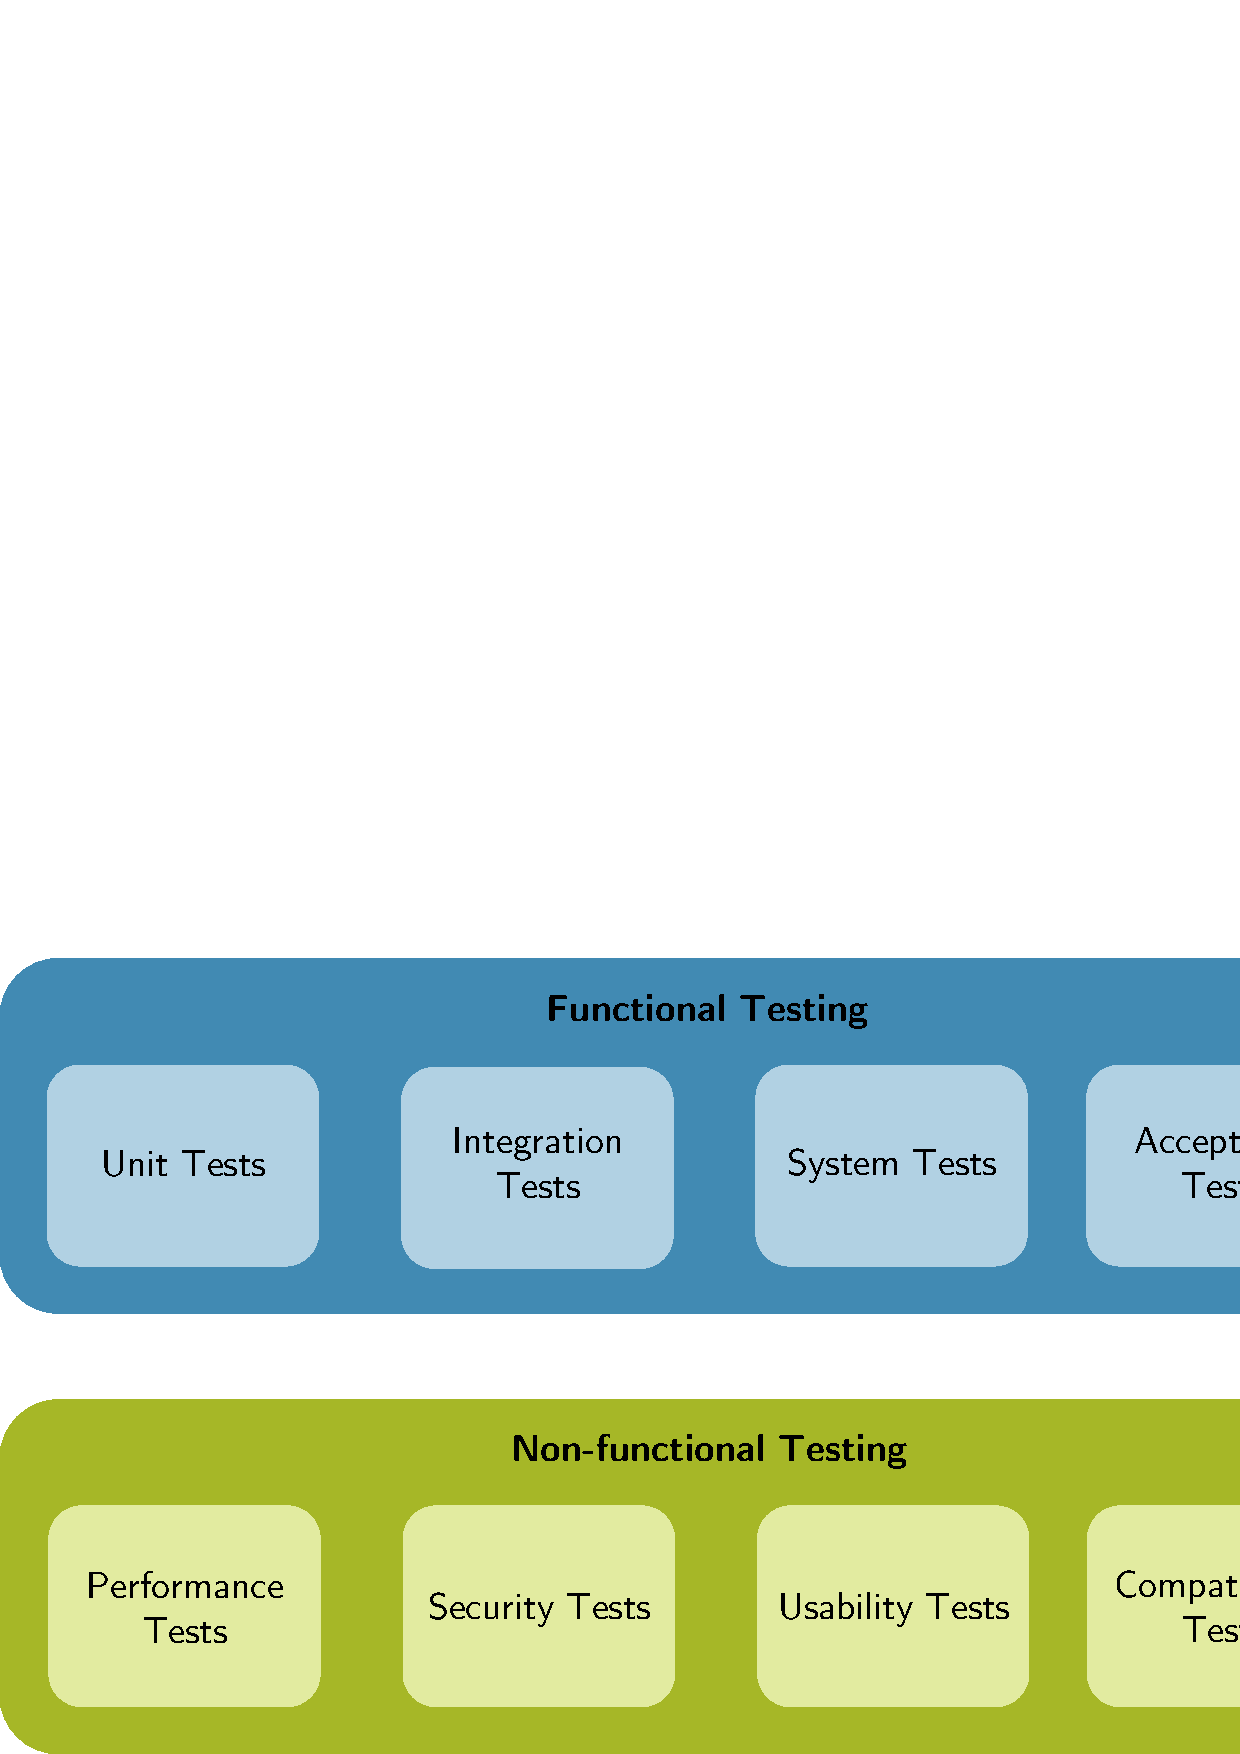
\includegraphics[width=0.9\linewidth]{images/img_testmethods.pdf}
	\captionof{figure}[Testmethoden]{Testmethoden\cite{TODO}}
	\label{fig:img_testmethods}
\end{minipage}

detailiert funktionale tests

\vspace{1em}
\begin{minipage}{\linewidth}
	\centering
	\includegraphics[width=0.9\linewidth]{images/img_testmethods_functional.pdf}
	\captionof{figure}[Funktionale Testmethoden]{Funktionale Testmethoden}
	\label{fig:img_testmethods_functional}
\end{minipage}

\subsection{Testen von Microservices}

\paragraph{Unit Tests}

hier steht text

\vspace{1em}
\begin{minipage}{\linewidth}
	\centering
	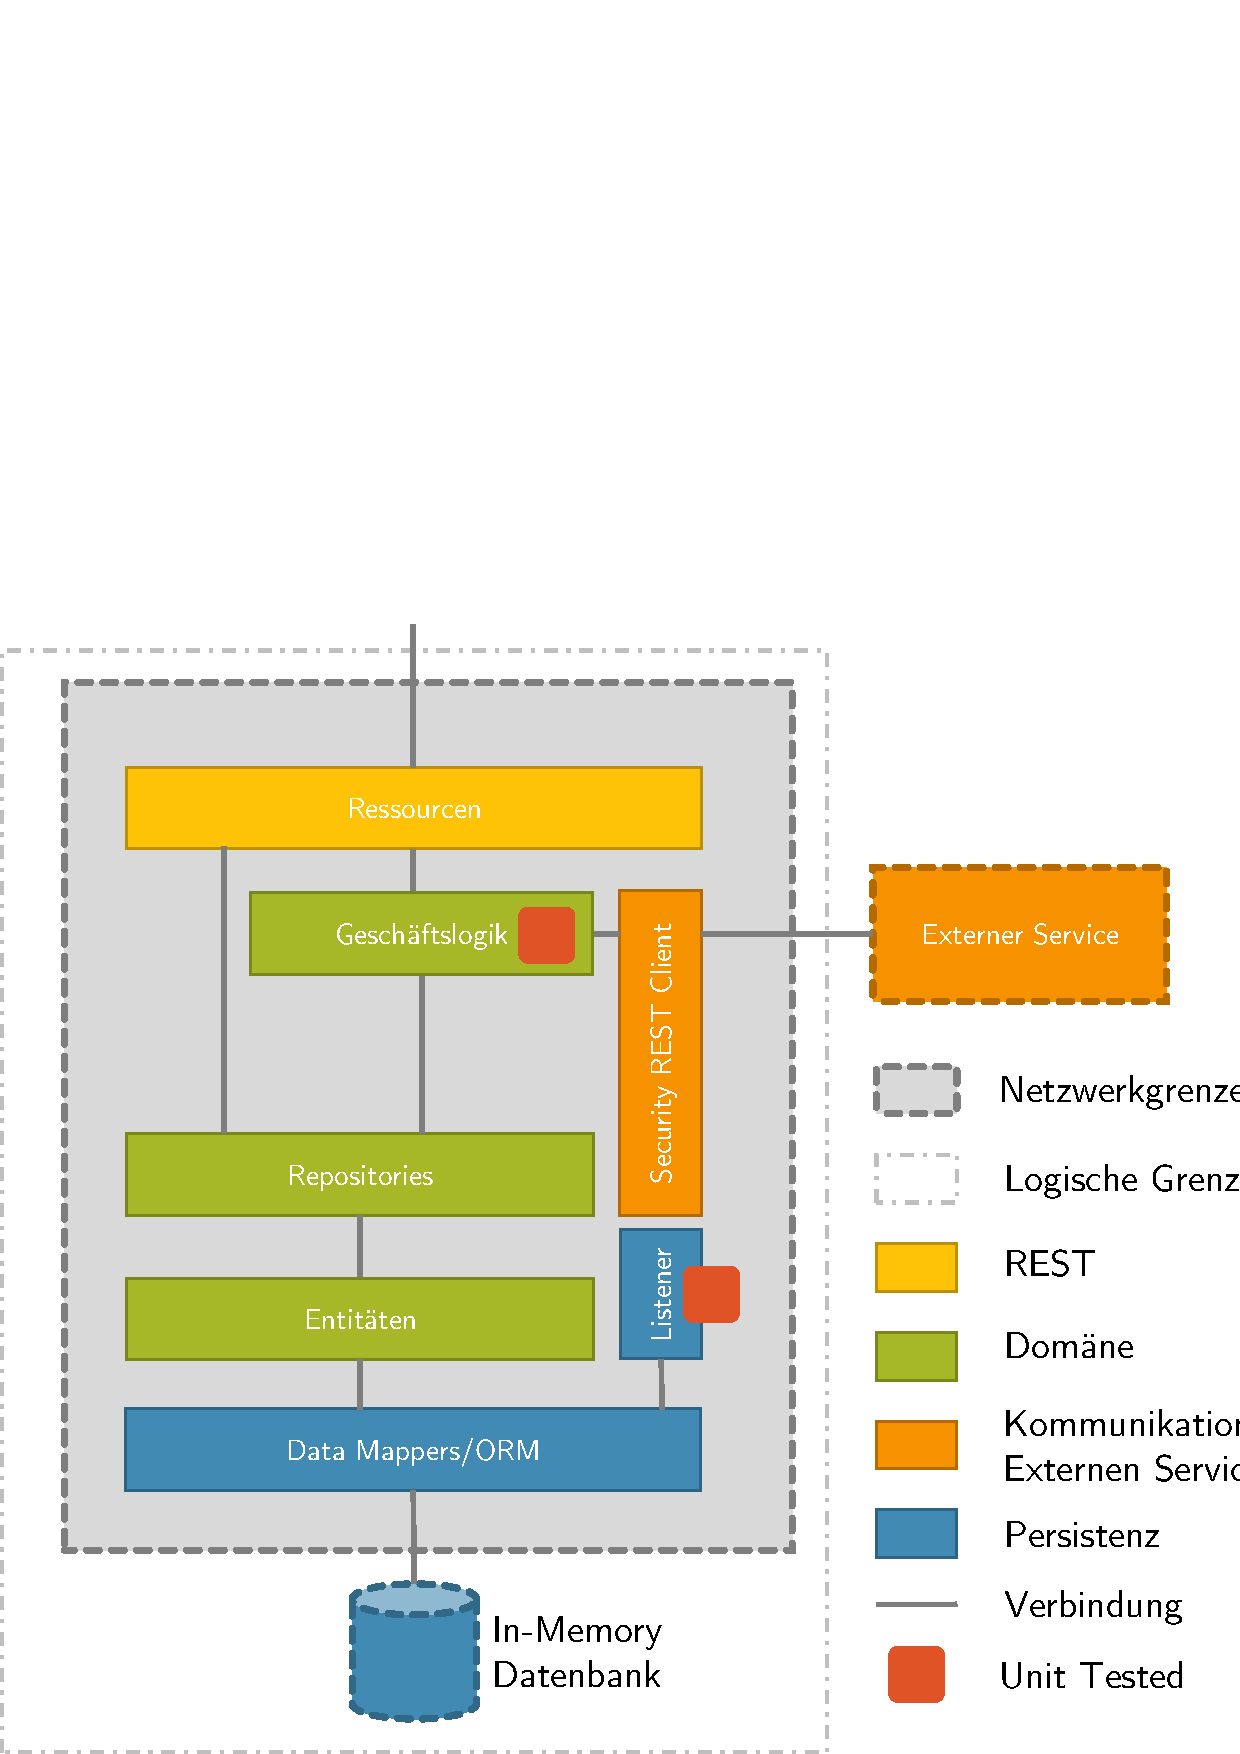
\includegraphics[width=0.9\linewidth]{images/img_unit-testing.PNG}
	\captionof{figure}[Unit Testing Scope]{Unit Testing Scope \cite{clemson}}
	\label{fig:img_unit-testing}
\end{minipage}

\paragraph{Integrationstests}

text

\vspace{1em}
\begin{minipage}{\linewidth}
	\centering
	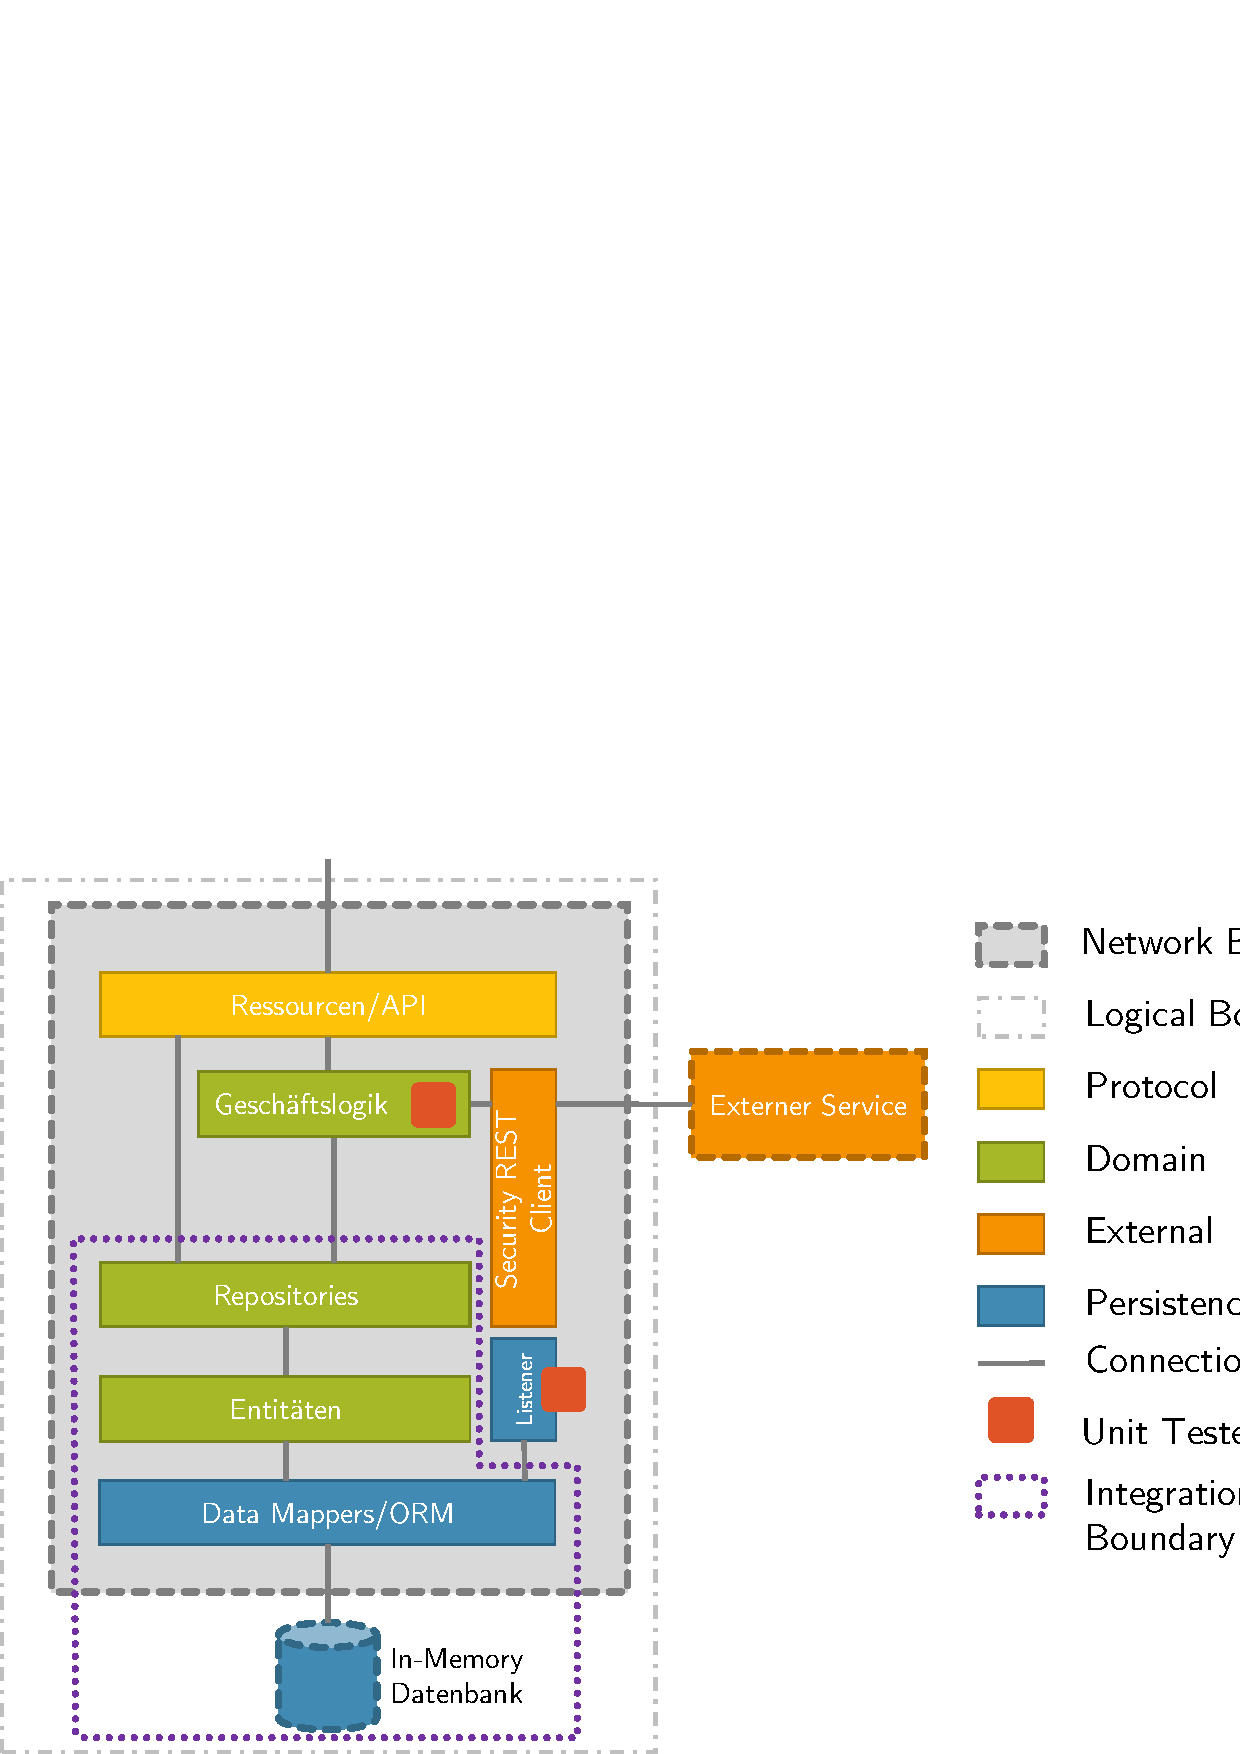
\includegraphics[width=0.9\linewidth]{images/img_integration-testing.PNG}
	\captionof{figure}[Integration Testing Scope]{Integration Testing Scope \cite{clemson}}
	\label{fig:img_integration-testing}
\end{minipage}

\paragraph{Komponententests}

text

\vspace{1em}
\begin{minipage}{\linewidth}
	\centering
	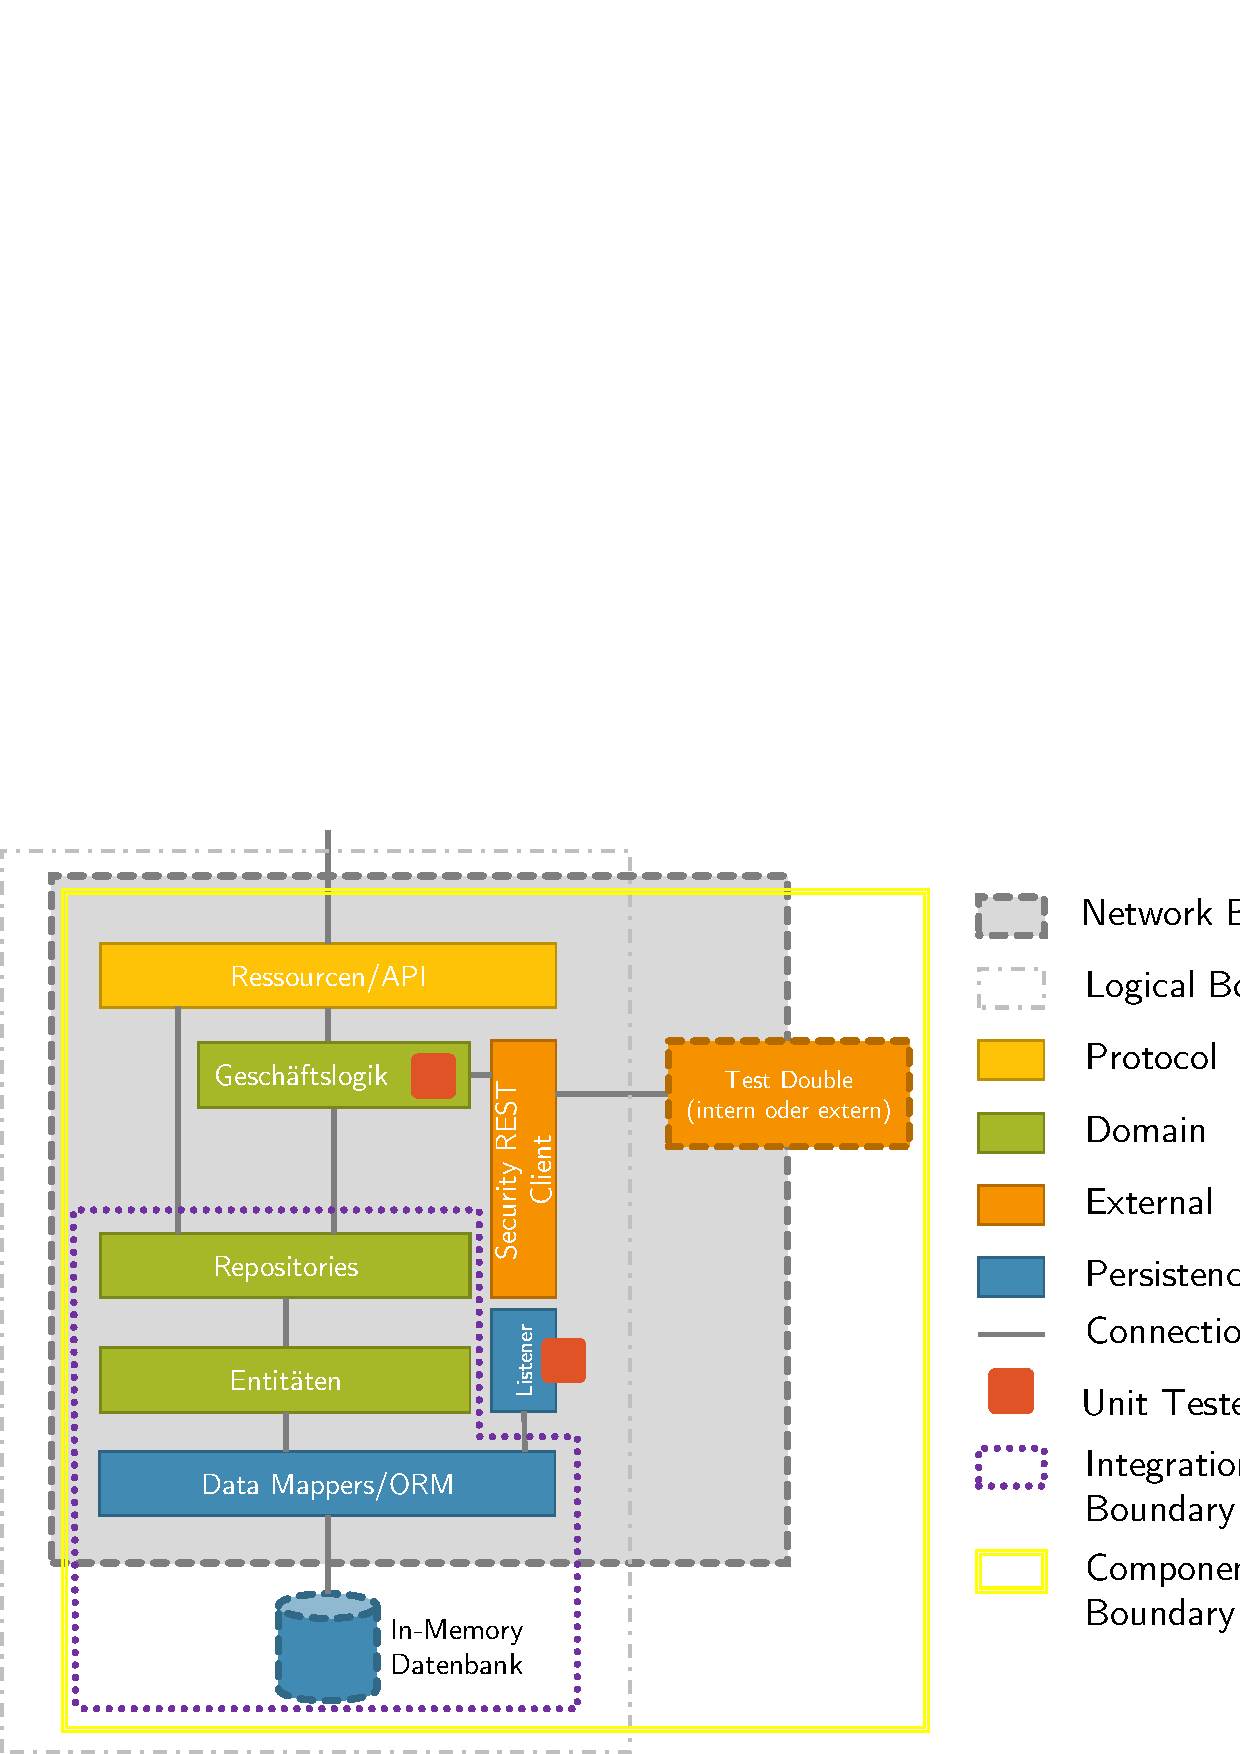
\includegraphics[width=0.9\linewidth]{images/img_component-testing.PNG}
	\captionof{figure}[Component Testing Scope]{Component Testing Scope \cite{clemson}}
	\label{fig:img_component-testing}
\end{minipage}

\paragraph{Contract Testing}

text

\vspace{1em}
\begin{minipage}{\linewidth}
	\centering
	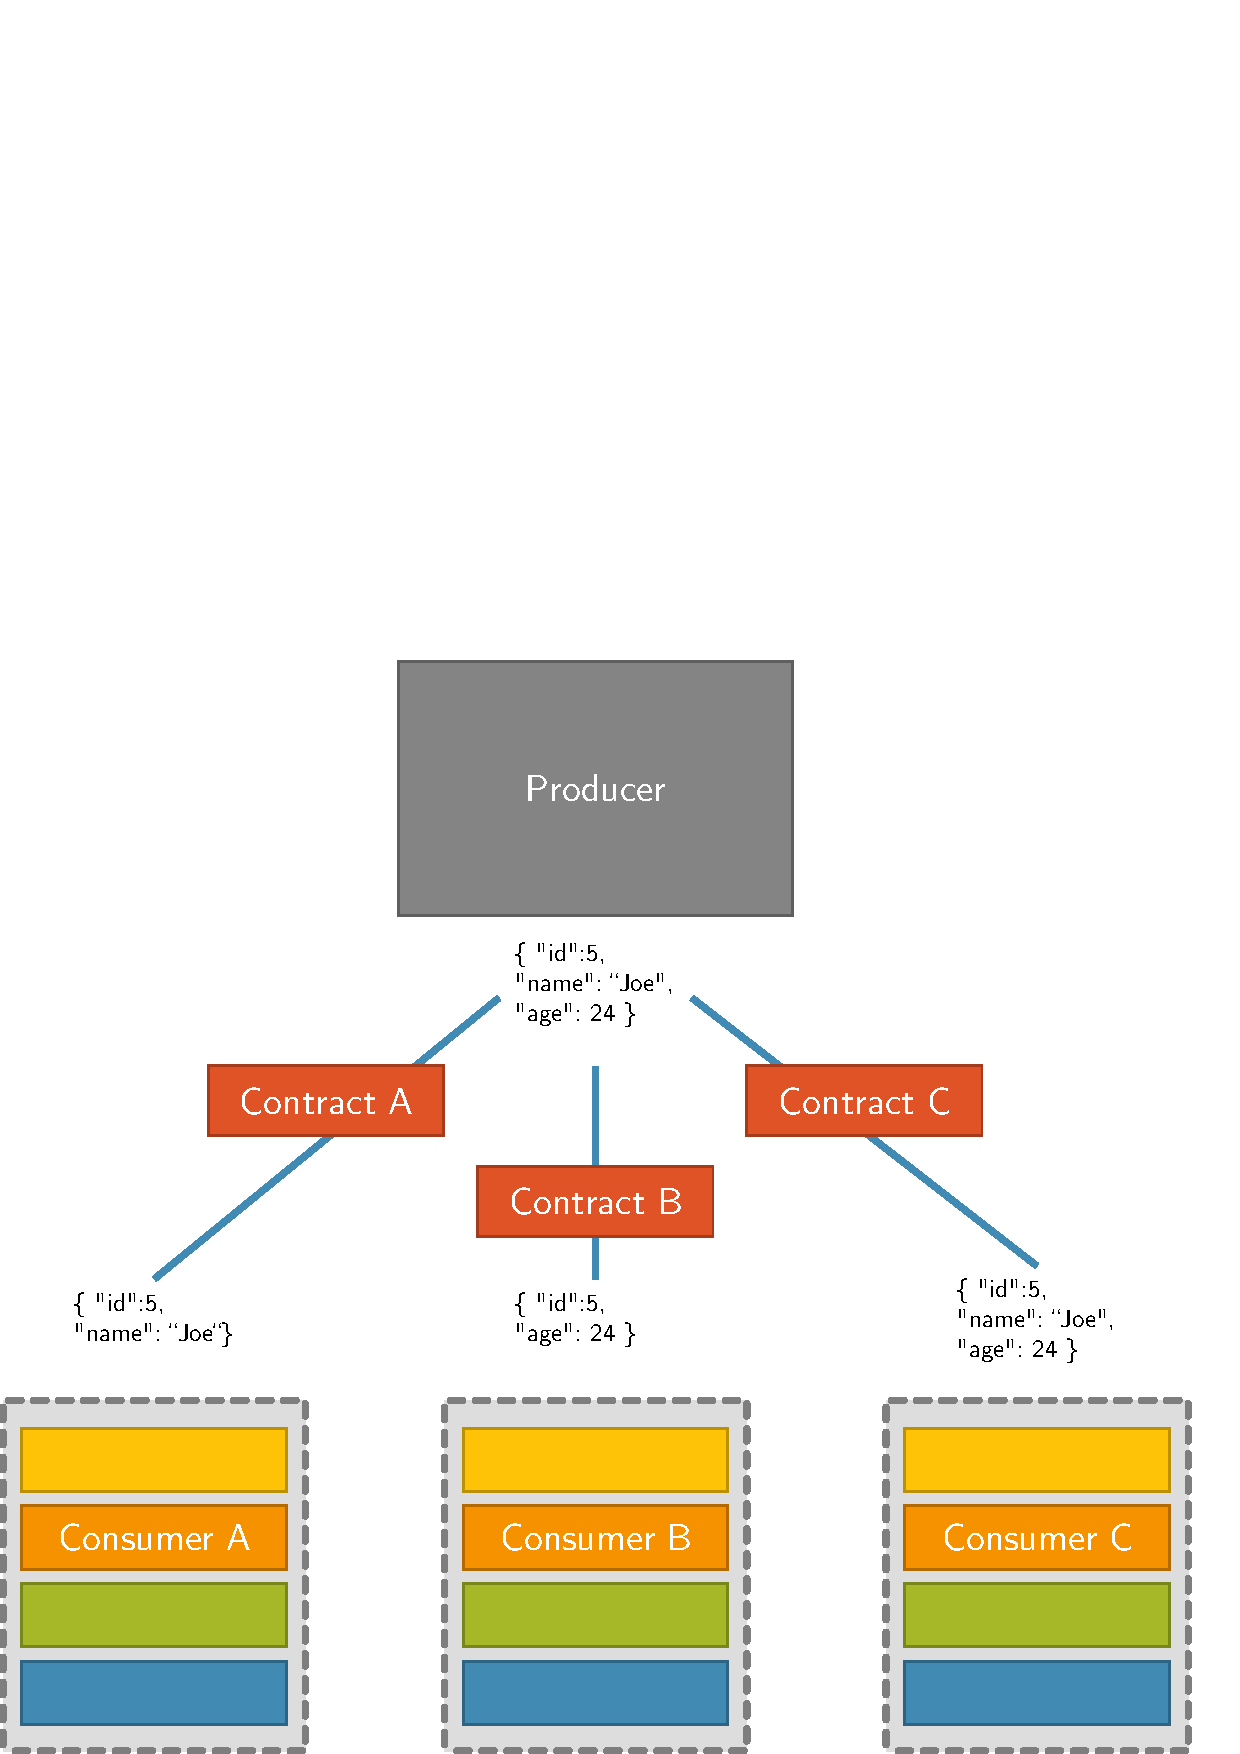
\includegraphics[width=0.9\linewidth]{images/img_contract-testing.PNG}
	\captionof{figure}[Contract Testing]{Contract Testing \cite{clemson}}
	\label{fig:img_contract-testing}
\end{minipage}

\paragraph{End-To-End Testing}

text

\vspace{1em}
\begin{minipage}{\linewidth}
	\centering
	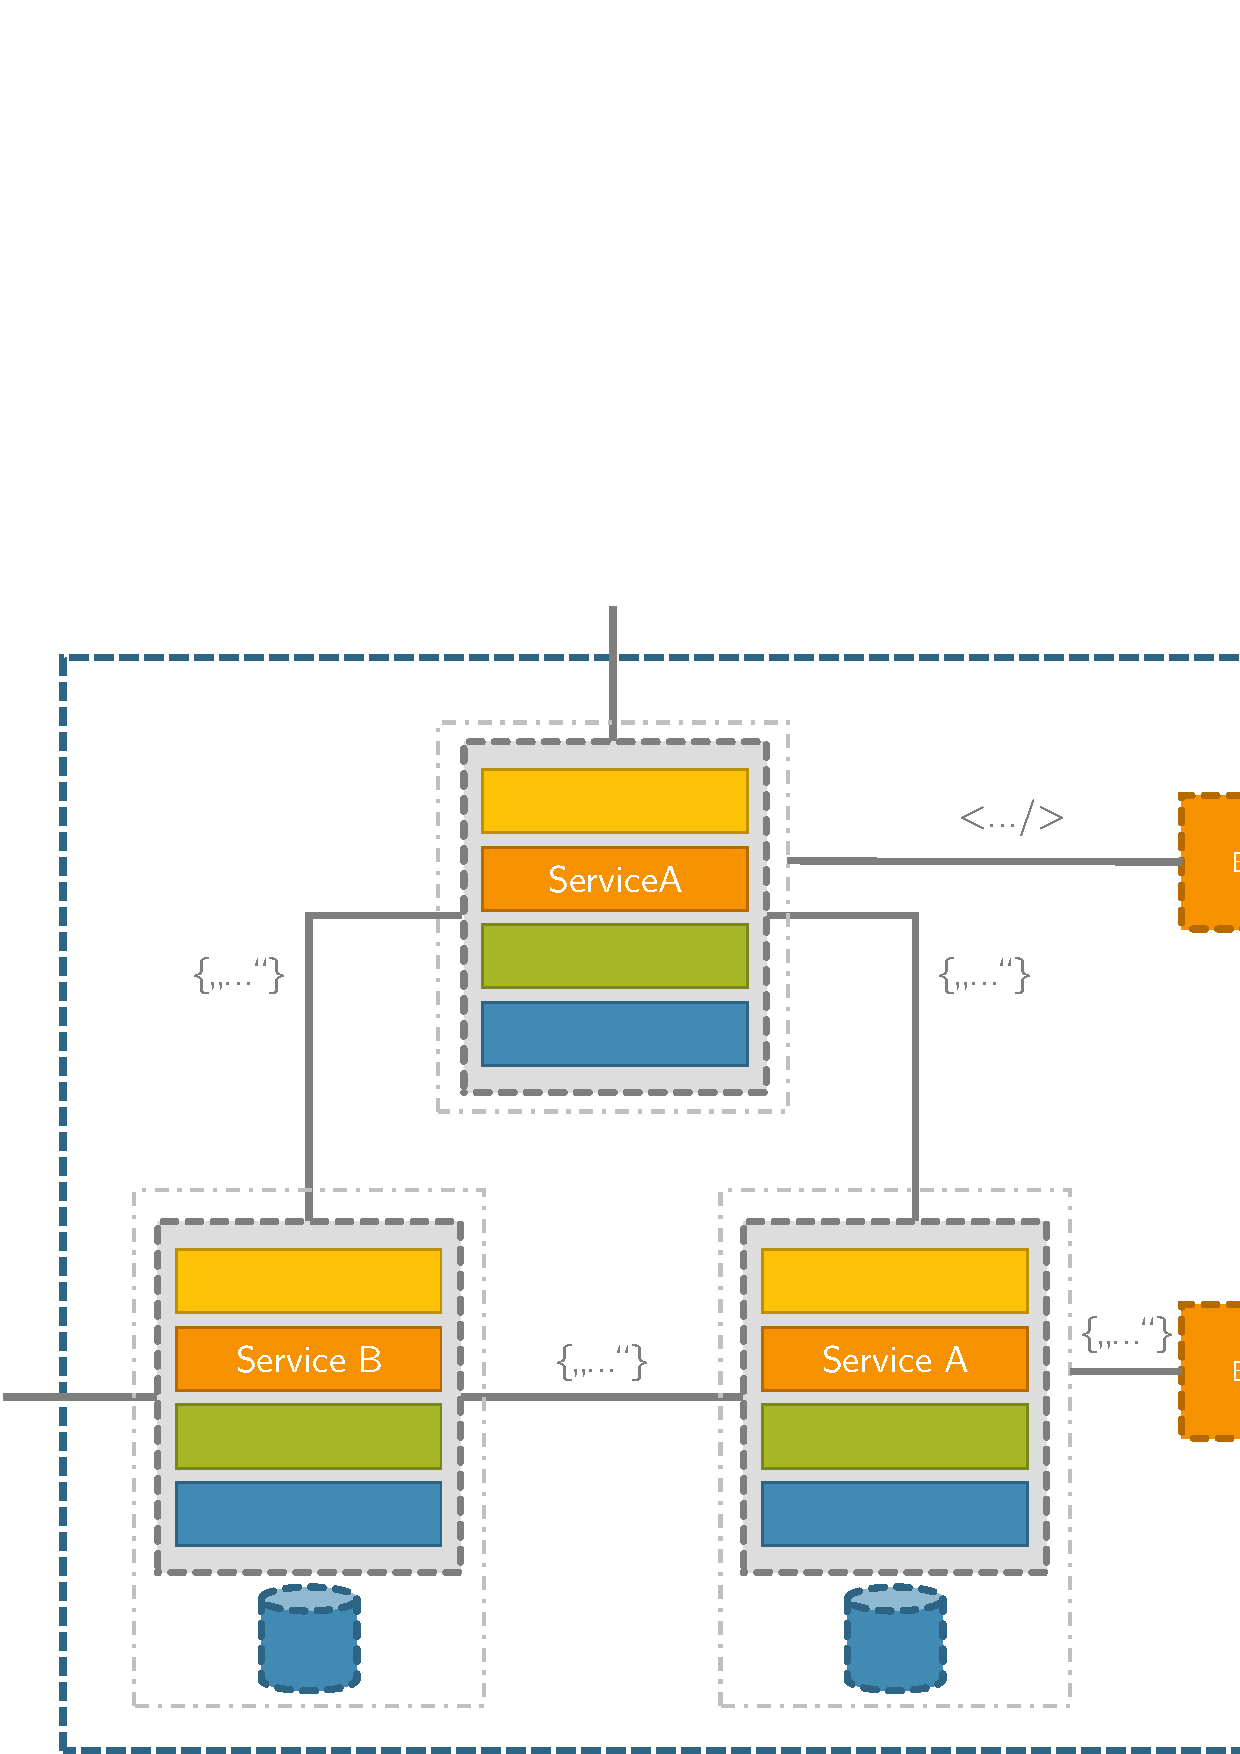
\includegraphics[width=0.9\linewidth]{images/img_end-to-end-testing.PNG}
	\captionof{figure}[End-To-End Testing Scope]{End-To-End Testing Scope \cite{clemson}}
	\label{fig:img_end-to-end-testing}
\end{minipage}

\subsubsection{Sinnvolle Teststrategien für den generativen Ansatz}

\subsubsection{Frameworks zum Umsetzen von Test-Strategien}

% ----------------------------------------------------------------------------------------------------------
% Architektur-Generierung für Software-Projekte
% ----------------------------------------------------------------------------------------------------------
\section{Architektur}

\subsection{Microservice Architektur und Unterschiede zur monolithischen Architektur}

\vspace{1em}
\begin{minipage}{\linewidth}
	\centering
	\includegraphics[width=0.9\linewidth]{images/img_monolithic-arch.PNG}
	\captionof{figure}[Monolithische Architektur]{Monolithische Architektur \cite{dinh}}
	\label{fig:img_monolithic-arch}
\end{minipage}

\vspace{1em}
\begin{minipage}{\linewidth}
	\centering
	\includegraphics[width=0.9\linewidth]{images/img_microservice-arch.PNG}
	\captionof{figure}[Microservice Architektur]{Microservice Architektur \cite{dinh}}
	\label{fig:img_microservice-arch}
\end{minipage}

\subsection{Vorgegebene Architektur der LHM}



\subsubsection{Authentifizierungsservice}

\subsubsection{Discoveryservice}

\subsubsection{Configurationservice}

\subsubsection{Service}

\subsubsection{Webservice}

\subsection{Unterschiede zwischen Microservices und Monolith-Architekturen}

\subsubsection{Auswirkungen}

% ----------------------------------------------------------------------------------------------------------
% Anforderungen an generierte Tests
% ----------------------------------------------------------------------------------------------------------
\section{Anforderungen an generierte Tests}

\subsection{Benötigte Daten}

\subsection{Notwendige Änderungen/Erweiterungen von Barrakuda}

% ----------------------------------------------------------------------------------------------------------
% Implementierung in Barrakuda
% ----------------------------------------------------------------------------------------------------------
\section{Implementierung in Barrakuda}

\subsection{Referenz-System}

\subsubsection{Komponenten und Aufbau}

\subsubsection{Implementierung des Systems}

\subsubsection{Implementierung der Tests}

\subsection{Übernahme der Referenz-Implementierung in Barrakuda-Templates}

% ----------------------------------------------------------------------------------------------------------
% Literatur
% ----------------------------------------------------------------------------------------------------------
\renewcommand\refname{Quellenverzeichnis}
\bibliographystyle{bibstyle}
\bibliography{bibfile}
\pagebreak

% ----------------------------------------------------------------------------------------------------------
% Anhang
% ----------------------------------------------------------------------------------------------------------
\pagenumbering{Roman}
\setcounter{page}{1}
\lhead{Anhang \thesection}

\begin{appendix}
\section*{Anhang}
\phantomsection
\addcontentsline{toc}{section}{Anhang}
\addtocontents{toc}{\vspace{-0.5em}}

\section{Code-Fragmente}
Viel Beispiel-Code

\end{appendix}

\end{document}
